\documentclass[UTF8,a4paper]{article}
\usepackage{fancyhdr}
\usepackage{ctex}
\usepackage{CJK}
\usepackage{amsmath}
\usepackage{listings}
\usepackage{graphics}
\usepackage{graphicx}
\usepackage{color}
\usepackage{xcolor}
\usepackage{geometry}
\usepackage{indentfirst}
\setlength{\parindent}{2em}
\geometry{left=1.5cm,right=1.5cm,top=2cm,bottom=1.5cm}
\lstset{breaklines}%这条命令可以让LaTeX自动将长的代码行换行排版
\lstset{extendedchars=false}%这一条命令可以解决代码跨页时,章节标题,页眉等汉字不显示的问题
\lstset{ 
	language=C++,                % choose the language of the code
	basicstyle=\small\sf,    % the size of the fonts that are used for the code
	tabsize=3,                            % sets default tabsize to 3 spaces
	numbers=left,                   % where to put the line-numbers
	numberstyle=\tiny,              % the size of the fonts that are used for the line-numbers
	stepnumber=1,                   % the step between two line-numbers. If it's 1 each line
	% will be numbered
	numbersep=5pt,                  % how far the line-numbers are from the code   %
	keywordstyle=\color[RGB]{33,33,234},               % keywords
	commentstyle=\color[RGB]{0,0,0},    % comments
	stringstyle=\color[rgb]{0.170,0.187,0.102},      % strings
    backgroundcolor=\color{white},
    rulesepcolor=\color[RGB]{20,20,20},  % choose the background color. You must add \usepackage{color}
	showspaces=false,               % show spaces adding particular underscores
	showstringspaces=false,         % underline spaces within strings
	showtabs=false,                 % show tabs within strings adding particular underscores                frame = single,         % adds a frame around the code
	captionpos=b,                   % sets the caption-position to bottom
	breaklines=true,                % sets automatic line breaking
	breakatwhitespace=false,        % sets if automatic breaks should only happen at whitespace
	title=\lstname,                 % show the filename of files included with \lstinputlisting;
	% also try caption instead of title
	mathescape=true,escapechar=?    % escape to latex with ?..?
	escapeinside={\%*}{*)},         % if you want to add a comment within your code
	%columns=fixed,                  % nice spacing
	%morestring=[m]',                % strings
	%morekeywords={%,...},%          % if you want to add more keywords to the set
	%    break,case,catch,continue,elseif,else,end,for,function,global,%
	%    if,otherwise,persistent,return,switch,try,while,...},%
}
\pagestyle{fancy}
\lhead{数据结构作业}
\chead{}
\rhead{\bfseries 22920182204393庄震丰}
\lfoot{}
\cfoot{\thepage}
\rfoot{}
\renewcommand{\headrulewidth}{0.4pt}
\begin{document}
\begin{center}
    \textbf{\LARGE{数据结构作业 第六章}}\\[0.5cm]
    \normalsize{庄震丰 22920182204393}\\[0.3cm]
    \large{Oct. $25^{th}$, 2019}
\end{center}
\textbf{6-33}\\
    题目要求:假定用两个一维数组作为有n个结点的二叉树的存储结构,L[i]和R[i]分别指示结点i(i=1,2,...n)的左孩子和右孩子,0表示空,试写出一个算法判断u是否为v的子孙。\\
	算法分析:对于给定的u和v,从v开始向下递归搜索每个结点看是否为u,并用全局变量进行标记,如果v的子孙没有则会全部遍历,若找到则直接输出判断结果。
	\\
	时间复杂度为O(N),空间复杂度O(N).\\
	6-33.cpp
\begin{lstlisting}
	#include<bits/stdc++.h>
	using namespace std;
	#define maxn 1000
	int L[maxn+1]={0},R[maxn+1]={0};//建立L,R数组储存节点左右儿子
	bool flag=false;
	void getfa(int x,int target)//从v开始往下递归搜素儿子节点
	{
		if (x==target) {flag=true;return;}
			if (L[x]!=0) getfa(L[x],target);
			if (R[x]!=0) getfa(R[x],target);
	}
	int main()
	{
		int n;
		int v,u;
		cin>>n;
		for (int i=1;i<=n;i++)
			cin>>L[i]>>R[i];
		cin>>v>>u;
		getfa(v,u); 
		cout<<flag;
		return 0;
	}
\end{lstlisting}
\textbf{样例输入1}\\
12\\
2 3\\
6 7\\
8 9\\
10 11\\
12 0\\
0 0\\
0 0\\
0 0\\
0 0\\
0 0\\
0 0\\
2 10\\
\textbf{样例输出1}\\
1\\
\textbf{说明}\\
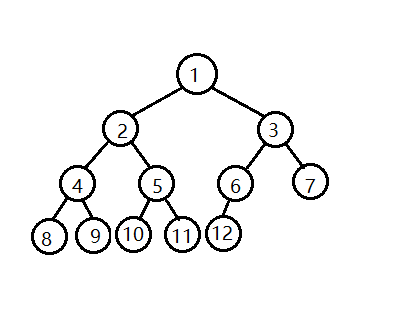
\includegraphics[width=0.7\textwidth]{6-33.png}\\
输入判断2是否为10的祖先,由图可知为真,输出1。\\\\
\textbf{6-62}\\
    题目要求:试编写算法,求一棵以孩子-兄弟表示的树,编写其深度的算法。\\
    算法分析:输入一棵双亲表示的树,运用机构提结点将其转换成孩子-兄弟表示法,再将其进行深搜,每从左结点递归则层数加一,最后统计最大值即可。\\
	时间复杂度O(n),空间复杂度O(n)。\\
	6-62.cpp
\begin{lstlisting}
	#include<bits/stdc++.h>
	using namespace std;
	#define maxn 1000
	#define inf 0x3f3f3f3f
	struct node
	{
		char name;
		node * lson;
		node * bro;
	};//孩子兄弟结构结点定义
	struct parentnode
	{
		int fa;
		char c;
		node * point;
	};//双亲数组结构结点定义
	parentnode A[maxn];
	int n;
	int cnt=1;
	node* trans()//将双亲数组结构转变成孩子兄弟树形结构
	{
		node * hp,*p1,*p2;
		hp=(node*)malloc(sizeof(node));
		hp->name=A[1].c;
		hp->bro=NULL;
		A[1].point=hp;//根节点单独判断
		for (int i=2;i<=n;i++)
			{
				if (A[i].fa!=A[i-1].fa) 
				{
					p1=(node*)malloc(sizeof(node));
					p1->bro=NULL;
					p1->lson=NULL;
					p1->name=A[i].c;
					A[i].point=p1;
					A[A[i].fa].point->lson=p1;
					//当前结点是新一层
				}
				else 
				{
					p2=(node *)malloc(sizeof(node));
					p2->bro=NULL;
					p2->lson=NULL;
					p2->name=A[i].c;
					A[i].point=p2;
					p1->bro=p2;
					p1=p2;//指针移动到兄弟结点
					//当前结点层数不变
				}
			}
		return hp;
	}
	void finddeep(node * p,int deep)//按照孩子-兄弟结构的指针进行遍历即可
	{
		cout<<p->name<<" ";
		if (p->bro==NULL&&p->lson==NULL) 
			{
				cnt=max(cnt,deep);
				
				return;
			}
		if (p->lson!=NULL) {finddeep(p->lson,deep+1);cout<<p->name<<" ";}
		if (p->bro!=NULL) {finddeep(p->bro,deep);cout<<p->name<<" ";}
		return;
	}
	bool cmp(parentnode a, parentnode b)
	{
		if (a.fa<b.fa) return true;
		else return false;
	}
	int main()
	{
		node * Heap;
		cin>>n;
		A[0].fa=-inf;
		for (int i=1;i<=n;i++)
		{ 
			scanf("%d %c",&A[i].fa,&A[i].c);//输入每个结点的父亲信息和该点的标号
		}
		sort(A+1,A+n+1,cmp);
			Heap=trans();//返回根节点指针
			finddeep(Heap,1);
			cout<<endl<<cnt;
		return 0;
	}
\end{lstlisting}
\textbf{样例输入一}\\
10\\
R -1\\
A 1\\
B 1\\
C 1\\
D 2\\
E 2\\
F 4\\
G 7\\
H 7\\
K 7\\
\textbf{样例输出一}\\
4\\
\textbf{样例说明}\\
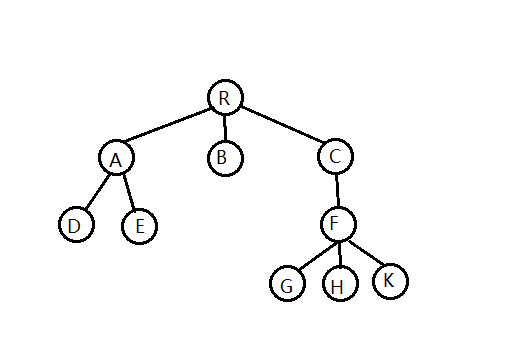
\includegraphics[width=0.5\textwidth]{6-62.png}
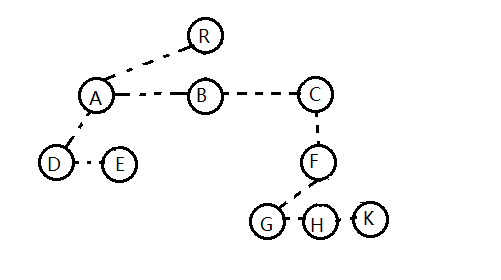
\includegraphics[width=0.5\textwidth]{6-62-1.png}
样例描述的树和孩子-兄弟表示法如图所示,层数为4。\\
\newpage
\noindent\textbf{6-65}\\
题目描述:已知一棵二叉树的前序和中序序列分别储存在两个一维数组中,试编写算法建立改树的二叉链表。\\
算法分析:先求树的结构,将其储存在一个数组中,在通过这个数组将其转变为链表形式,最后用后序遍历验证输出。\\
时间复杂度O(n),空间复杂度O(n)。\\
6-65.cpp
\begin{lstlisting}
	#include<bits/stdc++.h>
	using namespace std;
	#define maxn 1000
	#define inf 0x3f3f3f3f//设置无穷大
	struct node
	{
		char c;
		node *lson;
		node *rson;
	};//二叉链表结构体数组
	int n;
	node * hp;
	char Tree[maxn]={0};
	void work(string ptree,string mtree,int cnt)//将二叉树两种遍历转变成数组存储
	{
		char root=ptree[0];
		Tree[cnt]=root;
		if (ptree.length()!=1&&mtree.length()!=1)
		{
			int pos=mtree.find(root);
			work(ptree.substr(1,pos),mtree.substr(0,pos),cnt*2);
			work(ptree.substr(ptree.length()-pos,pos),mtree.substr(mtree.length()-pos,pos),cnt*2+1);
		}
		else
		{
			Tree[cnt]=root;
		}
		
	}
	void trans(int x,node * last,int size)//将数组变成二叉链表存储
	{
		node *p1;
		if (x==1) 
		{
			hp=(node *)malloc(sizeof(node));
			hp->lson=NULL;
			hp->rson=NULL;
			hp->c=Tree[x];
			if (Tree[x*2]) trans(x*2,hp,1);
			if (Tree[x*2+1]) trans(x*2+1,hp,2);
		}
		else
		{
			p1=(node *) malloc(sizeof(node));
			p1->lson=NULL;
			p1->rson=NULL;
			p1->c=Tree[x];
			if (Tree[x*2]) trans(x*2,p1,1);
			if (Tree[x*2+1]) trans(x*2+1,p1,2);
			if (size==1) last->lson=p1;
			else last->rson=p1;
		}
	}      
	void printlast(node * p)//后序遍历输出
	{
		
		if (p->lson==NULL && p->rson==NULL) return;
		if (p->lson!=NULL) printpre(p->lson);
		if (p->rson!=NULL) printpre(p->rson);
		cout<<p->c<<" ";
		return;
	}     
	int main()
	{
		cin>>n;
		string pre,mid;
		cin>>pre;
		cin>>mid;
		//初始化
		work(pre,mid,1);
		trans(1,NULL,0);
		printlast(hp);
	return 0;
	}
\end{lstlisting}
\textbf{样例输入1}\\
ABDECFG\\
DBEAFCG\\
\textbf{样例输出1}\\
DEBFGCA\\
(标准的三层二叉树)
\newpage
\noindent\textbf{6-37,38}\\
题目要求:用栈的基本操作写出先序遍历,后序遍历的非递归算法。\\
算法分析:先用数组存储树的结构,当栈不为空则一直进行操作,用vis进行标记某一节点是否遍历过,
如果当前栈顶(根)节点没有左右儿子则弹出栈pop,否则按照左右顺序依次入栈push。\\
后序遍历类似,但先是左右儿子入栈,不标记当前节点遍历,当左右儿子都弹出pop后标记当前top节点并输出。
时间复杂度O(N),空间复杂度O(N).\\
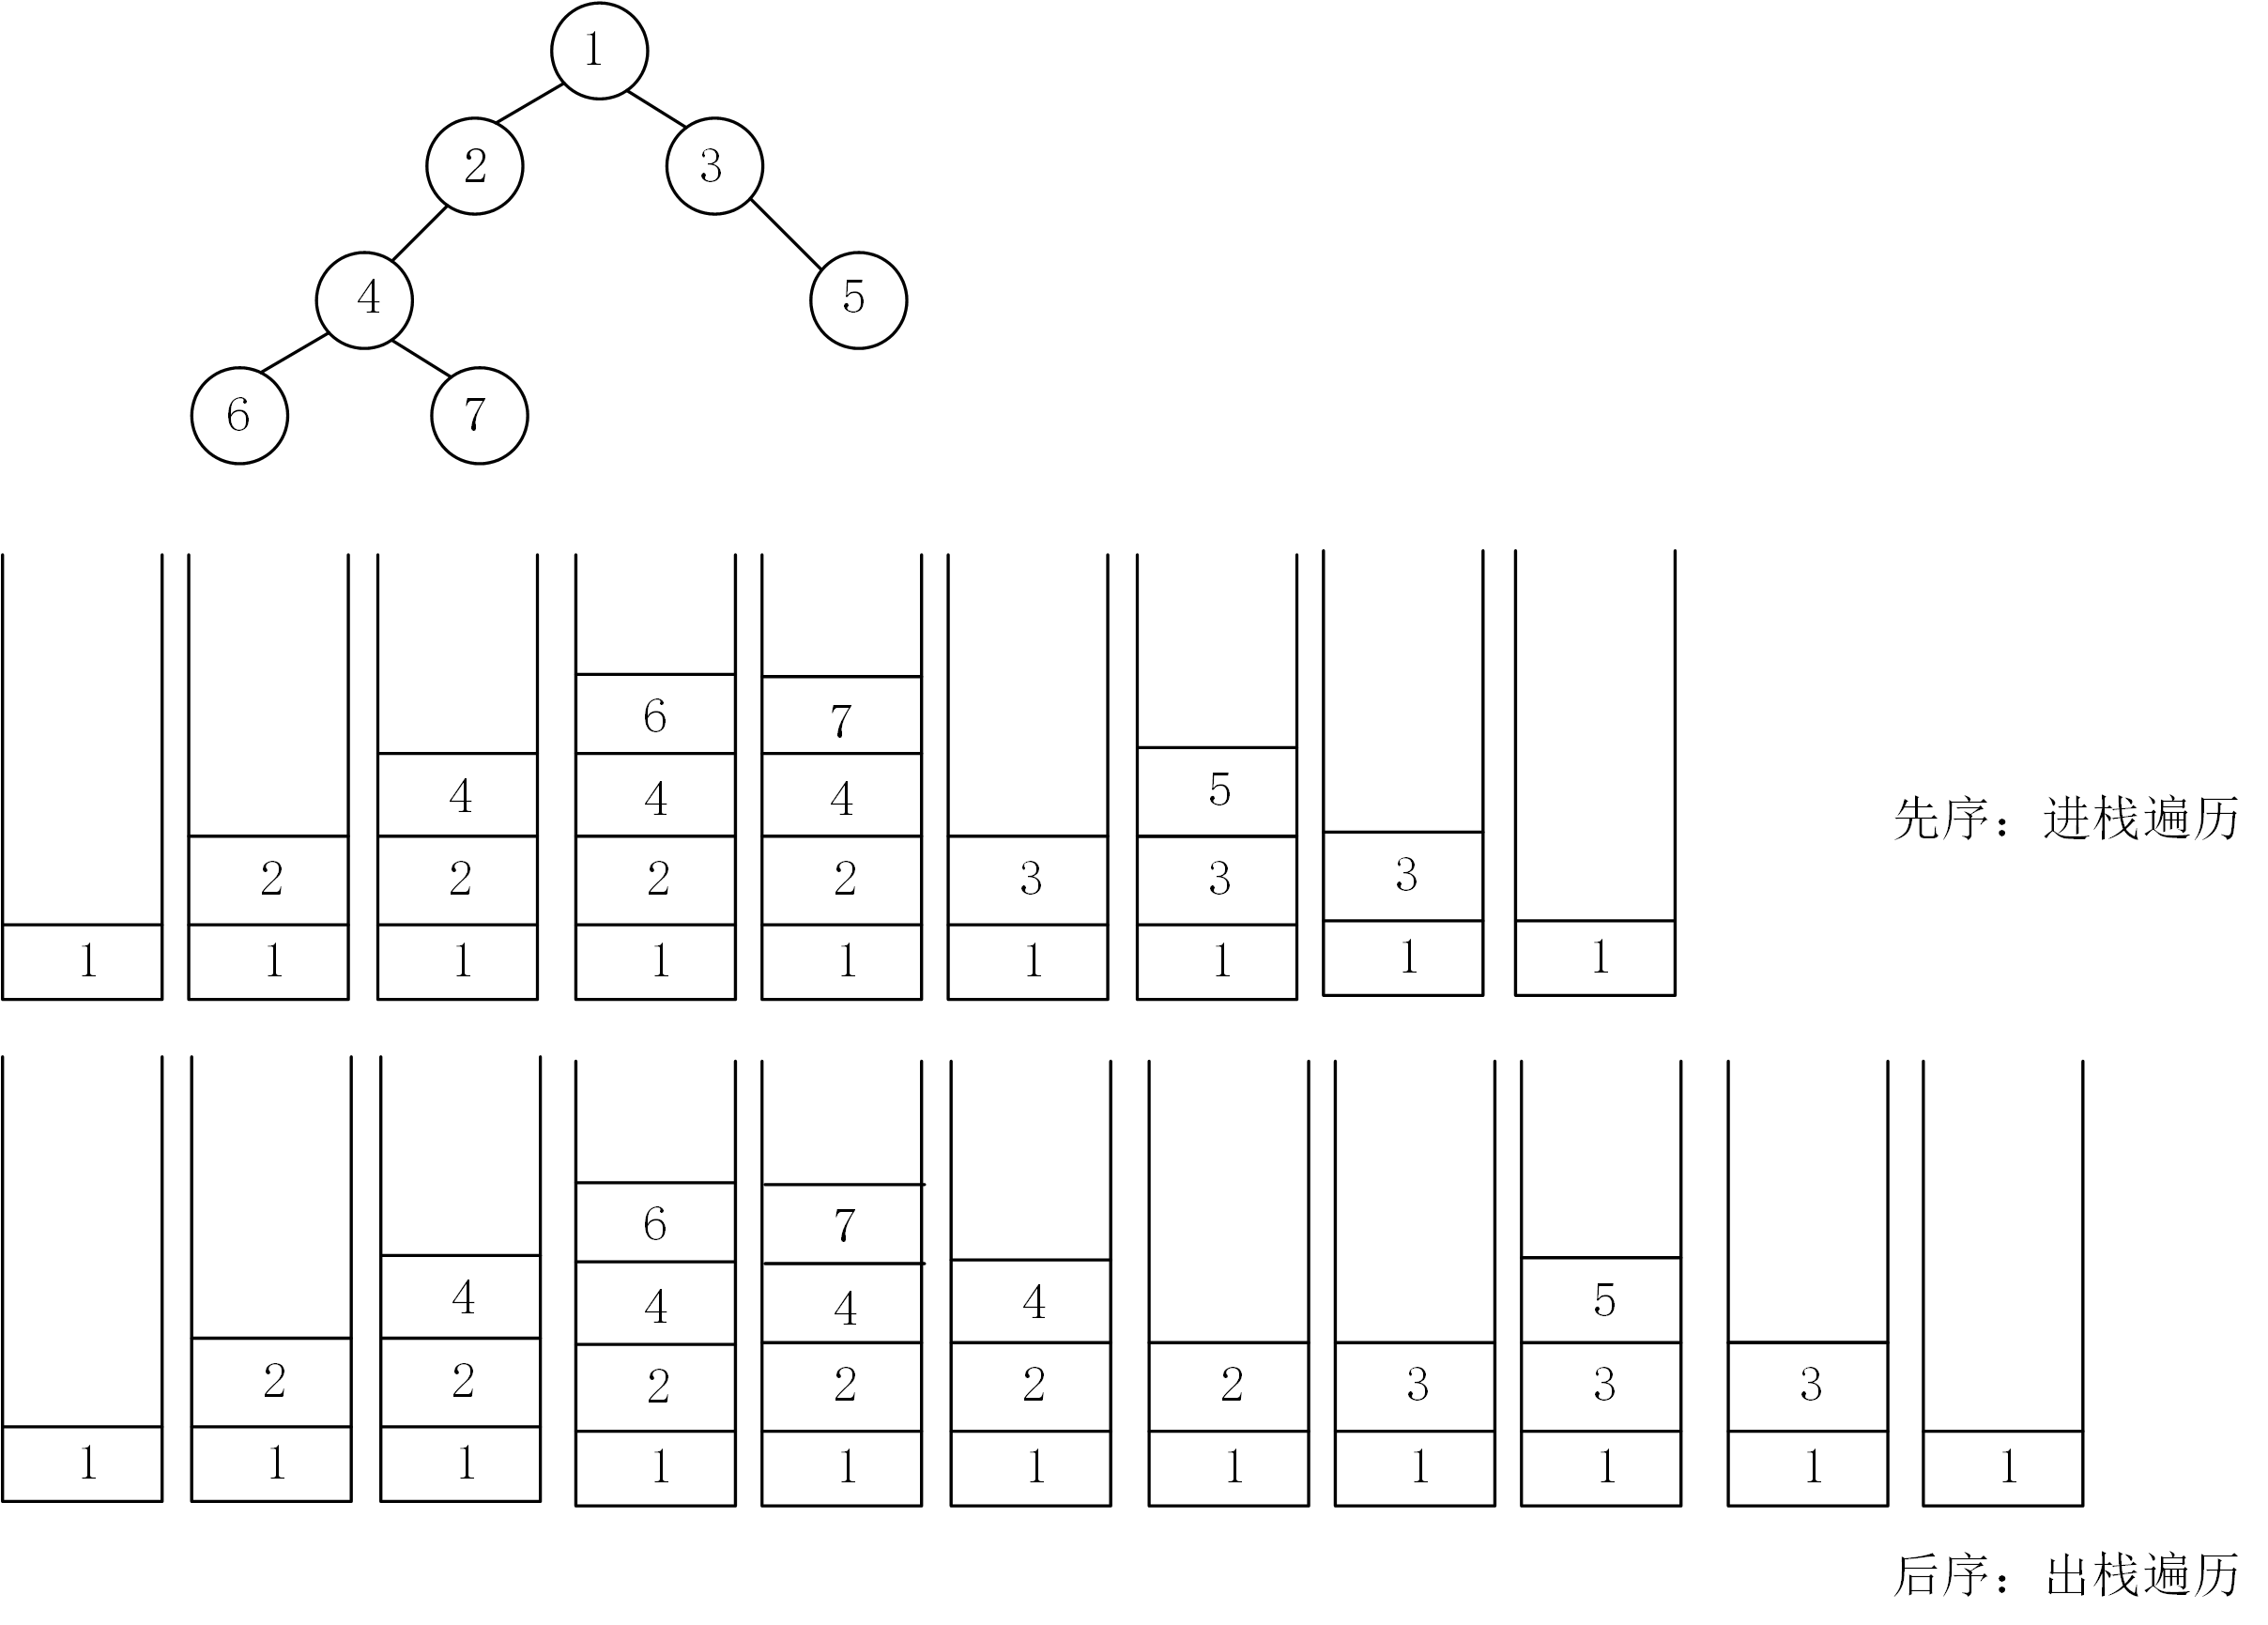
\includegraphics[scale=1]{6-37-38.png}
\textbf{code}
\begin{lstlisting}
	#include<bits/stdc++.h>
	#define maxn 1000
	using namespace std;
	int n;
	struct node
	{
		int num;
		int lson;
		int rson;
		bool vis;
		bool pri;
	}tree[maxn];
	stack<node> s;
	void pre_order()//先序遍历
	{
		while(!s.empty())//栈不为空则运行
		{
			if (!tree[s.top().num].vis)
			{
				cout<<s.top().num;
				tree[s.top().num].vis=true;
			}
			if  (s.top().lson==-1&&s.top().rson==-1)  s.pop();
			if (s.top().lson!=-1&&!tree[s.top().lson].vis) {//tree[s.top().lson].vis=true;                                                        s.push(tree[s.top().lson]);continue;}
			if (s.top().rson!=-1&&!tree[s.top().rson].vis) {//tree[s.top().rson].vis=true;
															s.push(tree[s.top().rson]);continue;}
			s.pop();
		}
	}
	void mid_order()//中序遍历
	{
		
		while(!s.empty())
		{
			if (s.top().lson==-1&&s.top().rson==-1)  {tree[s.top().num].vis=true;cout<<s.top().num;s.pop();}
			if (s.top().lson!=-1&&!tree[s.top().lson].vis) {s.push(tree[s.top().lson]);continue;}
			if (!tree[s.top().num].vis)
				{
				 cout<<s.top().num;
				 tree[s.top().num].vis=true;
				}
			if (s.top().rson!=-1&&!tree[s.top().rson].vis) {s.push(tree[s.top().rson]);continue;}
			s.pop();
		}
	}
	void last_order()//后序遍历
	{
		
		while(!s.empty())
		{
			if (s.top().lson==-1&&s.top().rson==-1)  {tree[s.top().num].vis=true;cout<<s.top().num;s.pop();}
			if (s.top().lson!=-1&&!tree[s.top().lson].vis) {tree[s.top().lson].vis=true;s.push(tree[s.top().lson]);continue;}
			if (s.top().rson!=-1&&!tree[s.top().rson].vis) {tree[s.top().rson].vis=true;s.push(tree[s.top().rson]);continue;}
			cout<<s.top().num;
			s.pop();
		}
	}
	
	int main()
	{
		int F,S,root;
		cin>>n;
		for (int i=1;i<maxn;i++)
		{
			tree[i].lson=-1;
			tree[i].rson=-1; 
			tree[i].vis=false;
		}
		for (int i=1;i<=n;i++)
		{
			int s_size;
	
			scanf("%d%d%d",&s_size,&F,&S);
			if (s_size==1) 
				tree[F].lson=S;
			else tree[F].rson=S;   
			tree[F].num=F;
			tree[S].num=S;
		}
		cin>>root;
		while(!s.empty()) s.pop();
		s.push(tree[root]);
		
		cout<<"pre-order:";
		pre_order();
		cout<<endl;
	
		for (int i=1;i<maxn;i++)
			tree[i].vis=false;
		tree[root].vis=true;
		s.push(tree[root]);
		
		cout<<"last-order:";
		last_order();
		cout<<endl;
	
		for (int i=1;i<maxn;i++)
		tree[i].vis=false;
		s.push(tree[root]);
		cout<<"mid-order:";
		mid_order();
	}
\end{lstlisting}
\textbf{6-43}
题目要求:编写递归算法,将二叉树的所有结点的左右子树互相交换。\\
算法分析:用数组结构体的形式表示二叉树,先根据输入信息建立数据关系,再递归从根节点到叶子节点进行翻转。\\
时间复杂度O(N),空间复杂度O(N).\\
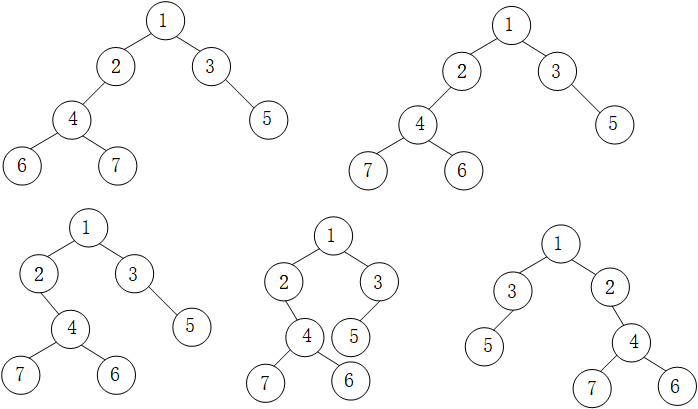
\includegraphics[scale=1]{6-43.png}\\
\textbf{Code}\\
\begin{lstlisting}
#include<bits/stdc++.h>
using namespace std;
#define maxn 1000
#define inf 0x3f3f3f3f
int n,root,Mnode=-inf;
struct innode//树结点
{
    char name;
    innode* l;//结点左儿子
    innode* r;//结点右儿子
}A[maxn],*p=A;

void rev(innode x)//翻转左右儿子
{
    *innode pn;
    if (x.l!=NULL)  rev(*(x.l));
    if (x.r!=NULL)  rev(*(x.r));
    pn=x.l;
    x.l=x.r;
    x.r=pn;
}
int main()
{
    cin>>n;
    cin>>root;
    int a,ls,rs;
    char c;
    for (int i=0;i<maxn;i++)
        {
            A[i].l=NULL;
            A[i].r=NULL;
        }
    for (int i=1;i<=n;i++)
    { 
        scanf("%d %d %d %c",&a,&ls,&rs,&c);//输入每个结点的父亲信息和该点的标号
        A[a].name=c;
        A[a].l=(p+ls);
        A[a].r=(p+rs);
    }
    rev(root);
 return 0;
}
\end{lstlisting}
\textbf{6-56}\\
题目要求:试写一个算法,再先序后继线索二叉树中,查找给定结点*p在先序序列中的后继。\\
算法分析:建立线索二叉树,若该节点没有右子树,则后继为p->rson.存在右子树,不存在左子树,则为p-rson。若存在左子树不存在右子树,则为p->lson。\\
时间复杂度O(N),空间复杂度O(N)。\\
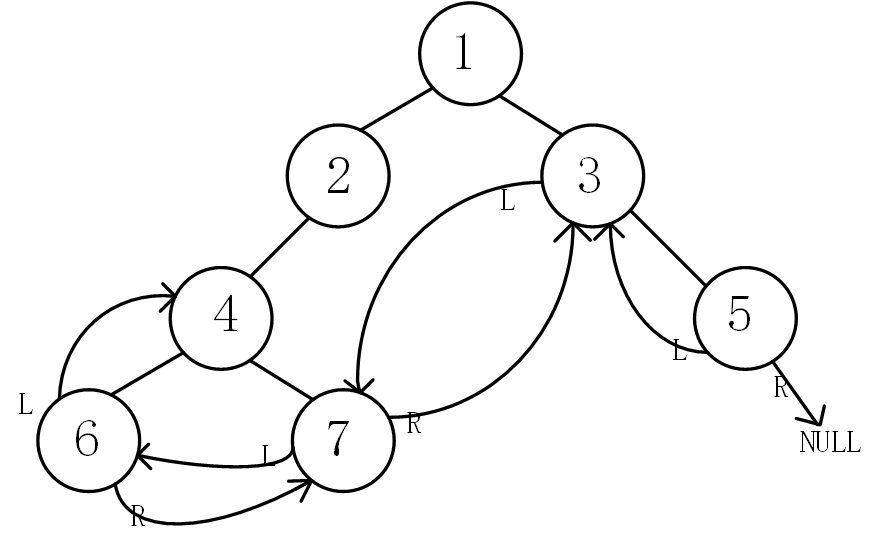
\includegraphics[scale=1.5]{6-56.png}\\
\textbf{Code}
\begin{lstlisting}
	#include<bits/stdc++.h>
	using namespace std;
	#define maxn 1000
	#define inf 0x3f3f3f3f
	int n,root;
	struct node//树结点
	{
		char name;
		node* ls;
		node* rs;
		int llog;
		int rlog;
		int num;
	};
	char A[maxn]={0};
	int n;
	node *heap=(node *)malloc(sizeof(node));//根节点
	void build(node * x)//建立一棵树
	{
		
		node *p1,*p2;//左右子树指针
		if (A[2*x->num]) 
		{
			x->llog=1;
			
			p1=(node*)malloc(sizeof(node));
			x->ls=p1;
			p1->ls=p1->rs=NULL;
			p1->name=A[2*x->num];
			p1->llog=p1->rlog=0;
			p1->num=2*x->num;
			build(p1);//左子树
		}
	   
		if (A[(2*x->num)+1]) 
		{
			x->rlog=1;
			p2=(node*)malloc(sizeof(node));
			x->rs=p2;
			p2->ls=p2->rs=NULL;
			p2->name=A[(2*x->num)+1];
			p2->llog=p2->rlog=0;
			p2->num=(2*x->num)+1;
			build(p2);//右子树
		}
	}
	node *P1,*P2;
	void oline(node * pf)//先序遍历将其线索化
	{
		P1=P2;
		P2=pf;
		if (P1->rs==NULL) P1->rs=pf;
		if (pf->ls==NULL) pf->ls=P1;
		if (pf->ls!=NULL) oline(pf->ls);
		if (pf->rs!=NULL) oline(pf->rs);
	}
	int main()
	{
		cin>>n;
		for (int i=0;i<maxn;i++)
			p[i]=NULL;
		for (int i=1;i<n;i++)
			cin>>A[i];//输入树节点信息
		heap->name=A[1];
		heap->llog=0;
		heap->rlog=0;//根初始化条件
		heap->num=1;
		build(heap);
		oline(heap);
		return 0;
	}
\end{lstlisting}	
\end{document}
